\section{Introduction}
Over the last decades the number of transistors on a chip is steadily rising (fig.~\ref{fig::moore}). Moore's Law is thereby the observation, that this number doubles roughly every 2 years \cite{moores_law}. Thus, the amount of functional units per chip rises at the same rate and this trend will probably continue.\\
However, hardware development capabilities do not scale with it. Therefore, development time increases, when using well-tried design methodologies. Thus, other methods are required, which limit the development time to a manageable amount. A suitable approach to this problem is to use a higher abstraction level to describe uniform structures. This is then used to generate all required parts of the module. Reducing the effort needed to design and maintain these components.\\
In this report a method is described to achieve this for a structure called register file (RF), which is often used in hardware designs. This tool is also used to simplify the development of multiple state of the art research projects containing RFs.
\begin{figure}[h]
 \centering
 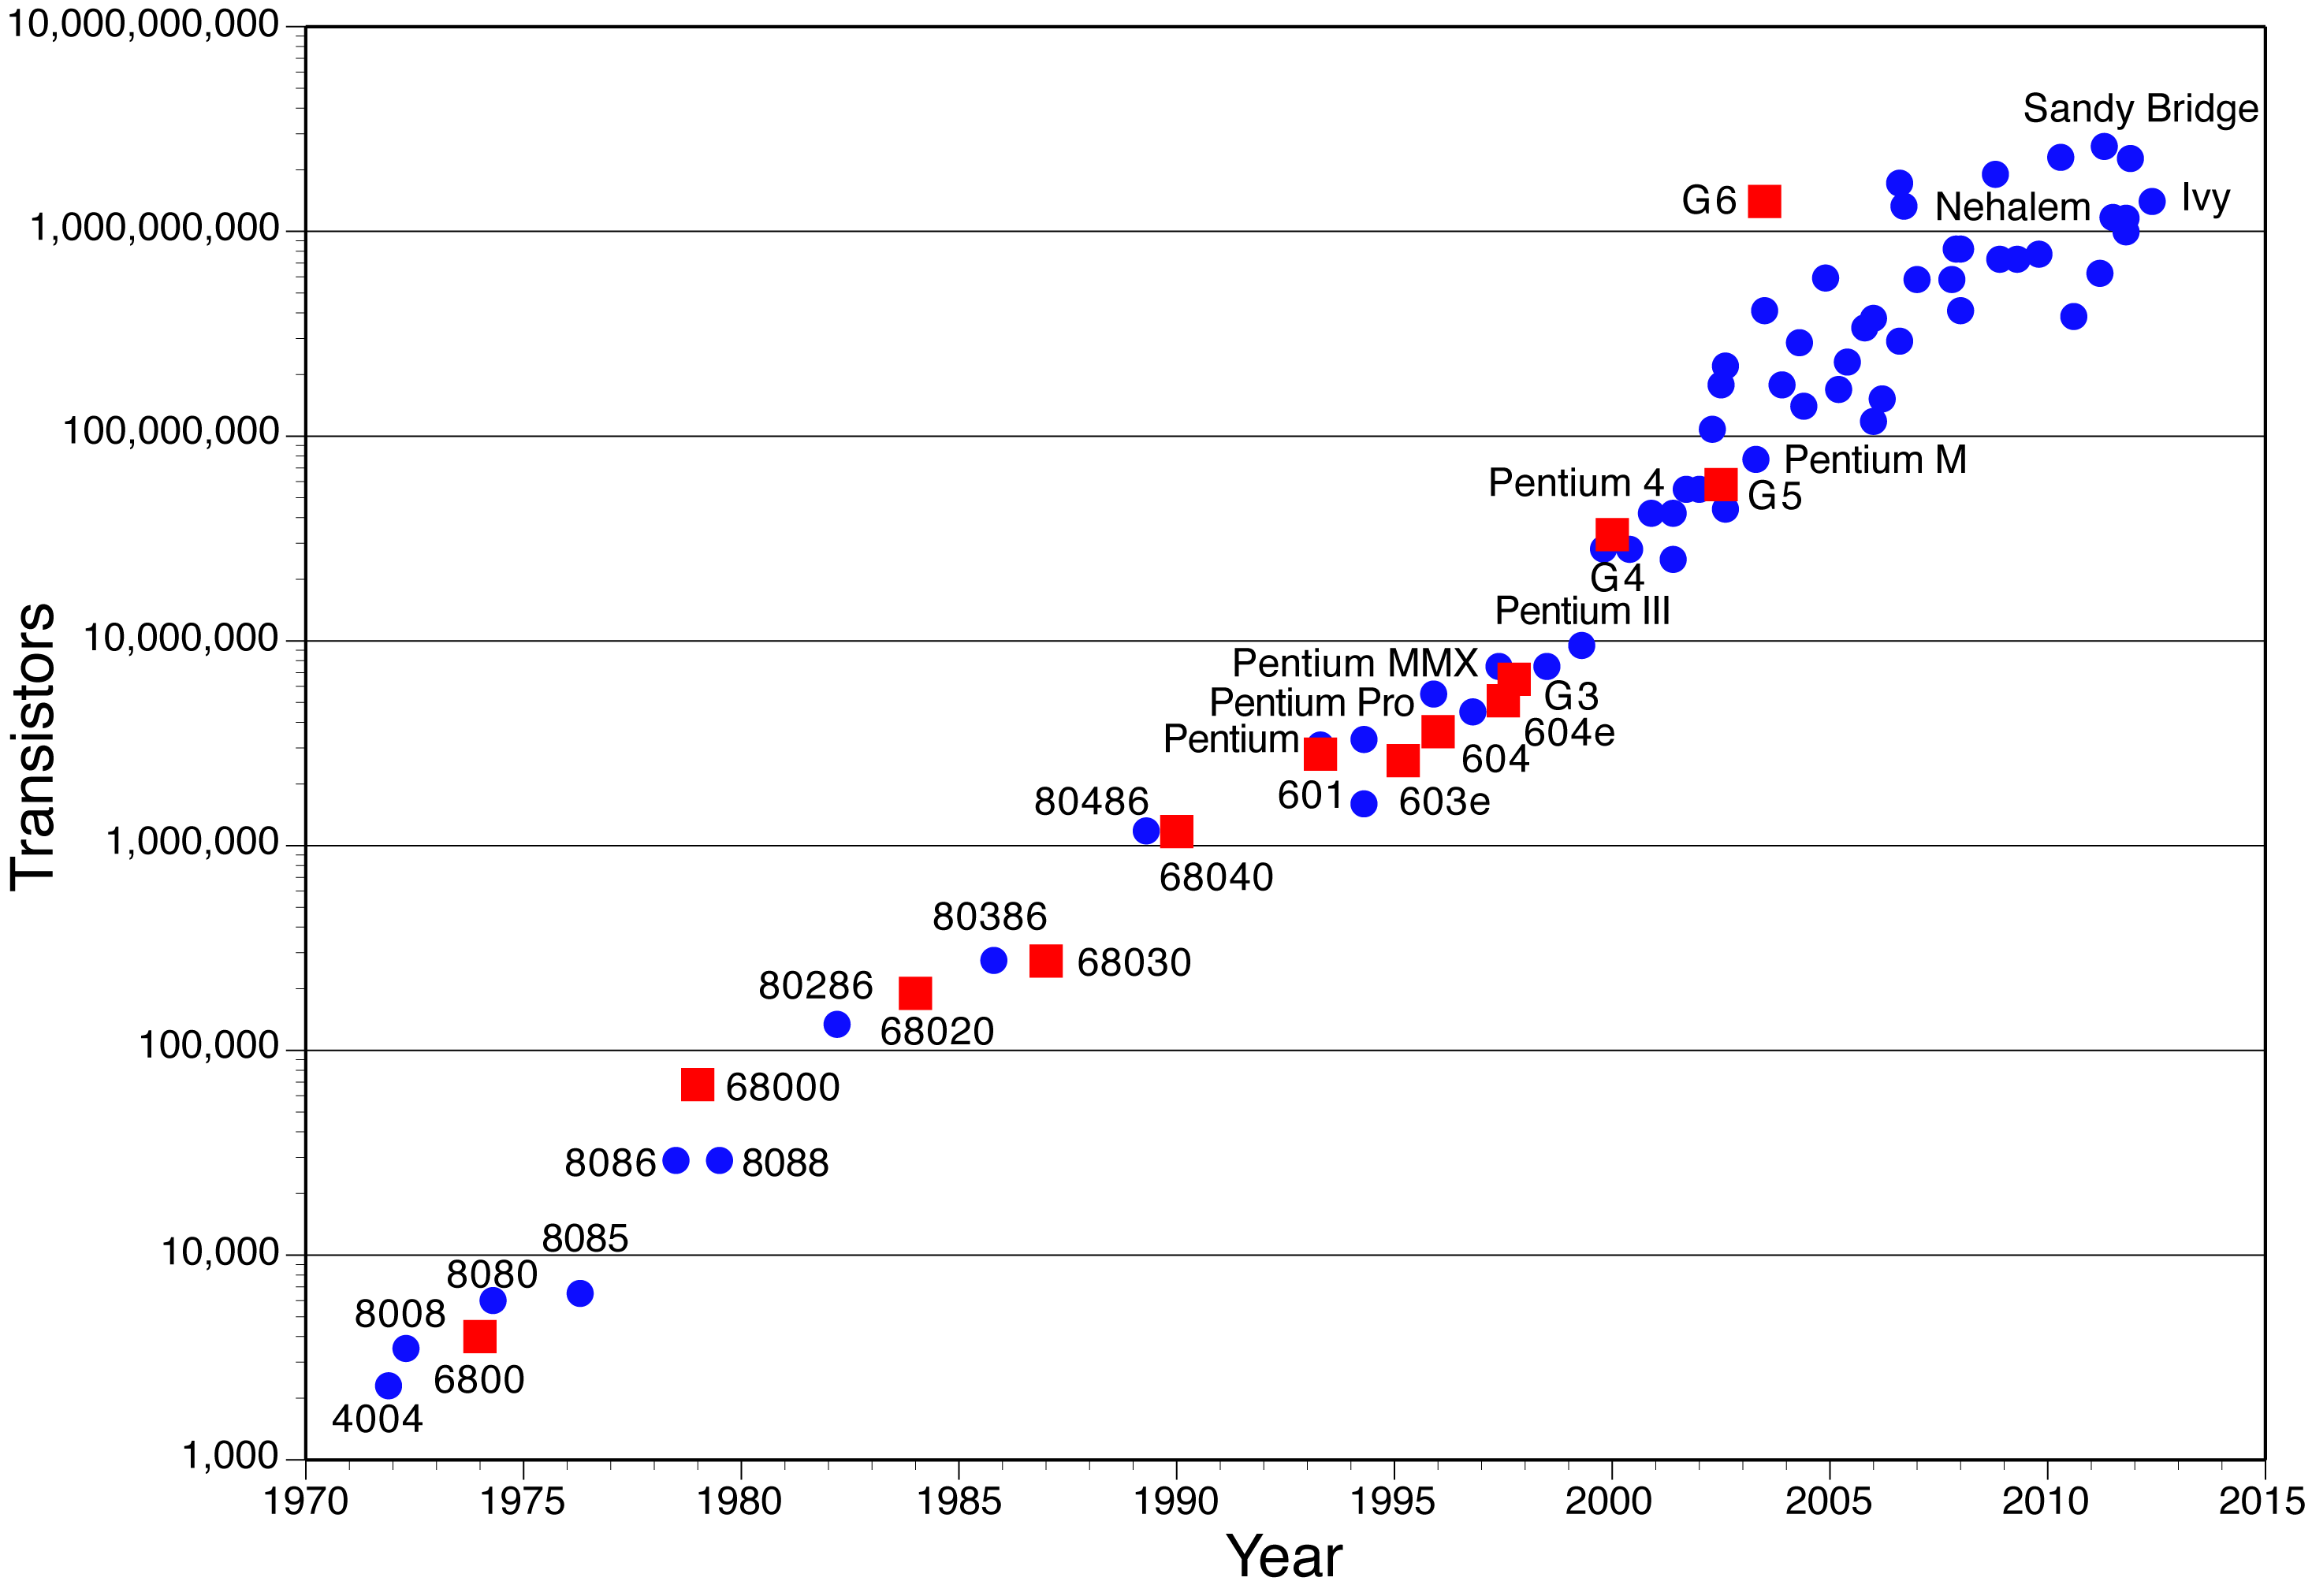
\includegraphics[width=252pt]{images/mooreslawcurve.png}
 \caption{Number of Transistors on a Chip \cite{moore}}
\label{fig::moore}
\end{figure}
